\documentclass[usenames,dvipsnames]{beamer}
\usepackage{mycommonstyle}

\title{Weighted Decision Tree}
\date{\today}
\author{Nipun Batra and teaching staff}
\institute{IIT Gandhinagar}

\begin{document}
	\maketitle
	
	

\begin{frame}

\begin{figure}
	\centering
	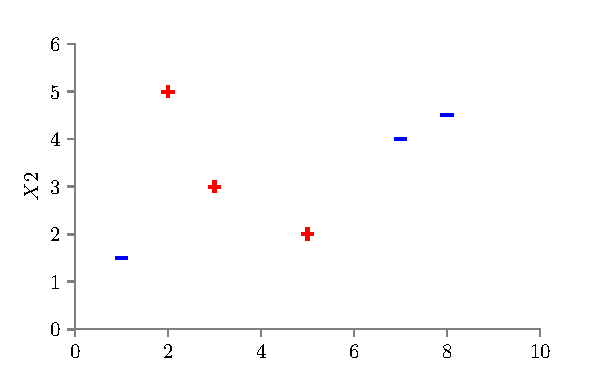
\includegraphics{../figures/dt_weighted/fig1.pdf}
\end{figure}


\end{frame}


\begin{frame}

\begin{figure}
	\centering
	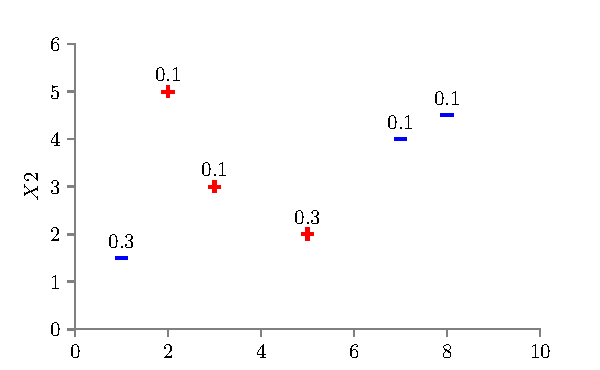
\includegraphics{../figures/dt_weighted/fig2.pdf}
\end{figure}


\end{frame}


\begin{frame}

\begin{figure}
	\centering
	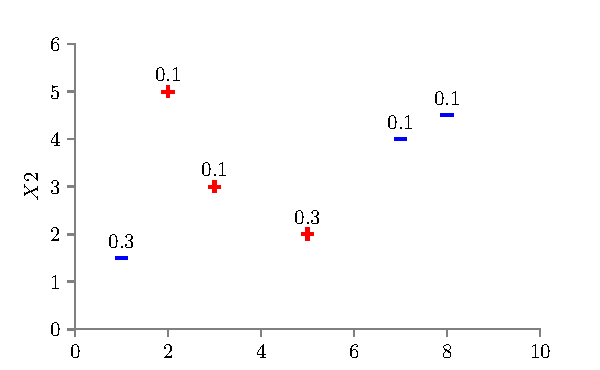
\includegraphics{../figures/dt_weighted/fig2.pdf}
\end{figure}

\(ENTROPY = - P(+) \cdot \log_2 P(+) - P(-) \cdot \log_2 P(-)\)

\(P(+) = \left( \frac{0.1 + 0.1 + 0.3}{1} \right) = 0.5\),      \(P(-) = \left( \frac{0.3 + 0.1 + 0.1}{1} \right) = 0.5\)

\(ENTROPY  = E_s =  - \frac{1}{2} \cdot log_2 \frac{1}{2}  - \frac{1}{2} \cdot log_2 \frac{1}{2}  = 1\)

\end{frame}





\begin{frame}

\begin{figure}
	\centering
	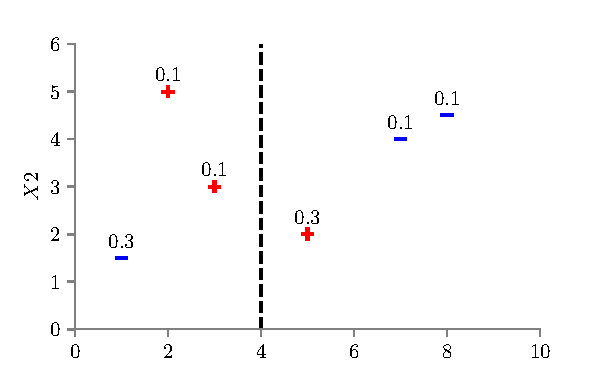
\includegraphics{../figures/dt_weighted/fig3.pdf}
\end{figure}

\(X1^* = 4\)


Candidate Line: \(X1 = X!^*\)


\end{frame}


\begin{frame}
\begin{figure}
	\centering
	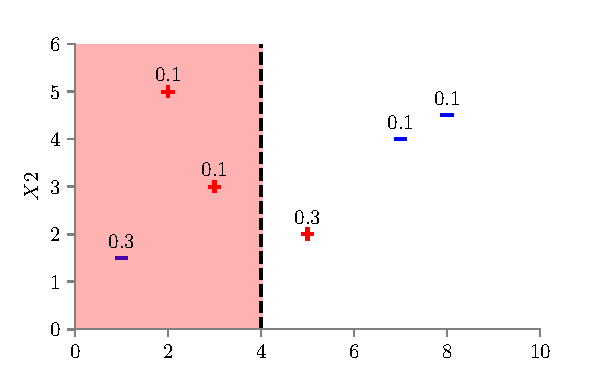
\includegraphics{../figures/dt_weighted/fig4.pdf}
\end{figure}

Entropy of \(X1 \leq X1^*  = E_{S(X1 < X1^*)}\)

\(P(+) = \left( \frac{0.1 + 0.1}{0.1 + 0.1 + 0.3} \right) = \frac{3}{5}\)

\(P(-) = \frac{3}{5}\)


\end{frame}


\begin{frame}

\begin{figure}
	\centering
	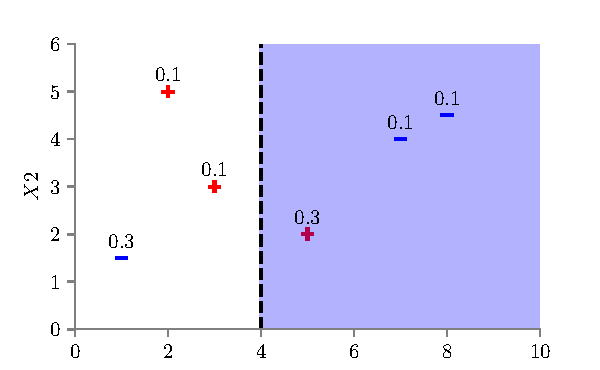
\includegraphics{../figures/dt_weighted/fig5.pdf}
\end{figure}
Entropy of \(X1  > X1^*  = E_{S(X1 > X1^*)}\)

\(P(+) = \left( \frac{3}{5} \right) = \frac{2}{5}\)

\(P(-) = \frac{3}{5}\)

\end{frame}



\begin{frame}

\begin{figure}
	\centering
	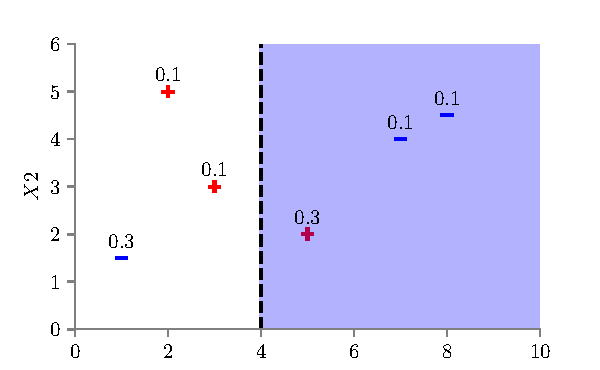
\includegraphics{../figures/dt_weighted/fig5.pdf}
\end{figure}

\( IG(X1 = X1^* ) = E_S - \frac{0.5}{1} \cdot E_{S(X1 < X1^*)}  - \frac{0.5}{1} \cdot E_{S(X1 > X1^*)}\)

\end{frame}

\end{document}